\documentclass [xcolor=svgnames, t] {beamer} 
\usepackage[utf8]{inputenc}
\usepackage{booktabs, comment} 
\usepackage[absolute, overlay]{textpos} 
\usepackage{pgfpages}
\usepackage[font=footnotesize]{caption}
\useoutertheme{infolines} 

\AtBeginSection[]{
  \begin{frame}
  \vfill
  \centering
  \begin{beamercolorbox}[sep=8pt,center,shadow=true,rounded=true]{title}
    \usebeamerfont{title}\insertsectionhead\par%
  \end{beamercolorbox}
  \vfill
  \end{frame}
}


%\definecolor{brownbrown}{RGB}{56, 28, 0}
%\definecolor{brownred}{RGB}{228, 0, 43}

%\setbeamercolor{title in head/foot}{bg=brownred, fg=brownbrown}
%\setbeamercolor{author in head/foot}{bg=myuniversity}
\setbeamertemplate{page number in head/foot}{}
\usepackage{csquotes}


\usepackage{amsmath}
\usepackage[makeroom]{cancel}
\usepackage[absolute,overlay]{textpos}

%\usepackage{textpos}

\usepackage{tikz}

\usepackage{media9} 

\usetheme{Madrid}
%\definecolor{myuniversity}{RGB}{56, 28, 0}
%\usecolortheme[named=myuniversity]{structure}
\usepackage{tikz}



\title[Viscosidad]{Clase No.12: Est\'atica de los fluidos}
\subtitle{Fuerzas sobre superficies planas, principios de flotaci\'on y equilibrio relativo de fluidos en movimiento}
\institute[]{Departamento de Ingenier\'ia Civil y Agr\'icola\\ Facultad de Ingenier\'ia  \\Universidad Nacional de Colombia - Sede Bogot\'a}
\titlegraphic{
\includegraphics[height=2.0cm]{escudoUnal.png}}
\author[LAM]{Luis Alejandro Morales \\ \href{https://lamhydro.github.io}{https://lamhydro.github.io}}


%\institute[]{Department of Earth, Environmental, and Planetary Sciences  \\Brown University}
\date{\today}


\addtobeamertemplate{navigation symbols}{}{%
    \usebeamerfont{footline}%
    \usebeamercolor[fg]{footline}%
    \hspace{1em}%
    \insertframenumber/\inserttotalframenumber
}

\begin{document}
\begin{frame}
\maketitle
\end{frame}


%%%%%%%%%%%%%%%%%%%%%%%%%%%%
\logo{\vspace{-0.2cm}
\includegraphics[height=0.8cm]{escudoUnal.png}~%
}
%%%%%%%%%%%%%%%%%%%%%%%%%%



\begin{frame}
\frametitle{Table of Contents}
\tableofcontents
\end{frame}

\section{Fuerzas sobre superficies curvas}
\begin{frame}{Fuerzas sobre superficies curvas: Aplicaciones}
Necesaria en la estimaci\'on de fuerzas sobre estructuras hidr\'aulicas curvas como:
\begin{itemize}
\item compuertas tipo tambor
\item compuertas radiales
\item Cara superior tipo par\'abola en presas
\end{itemize}
\begin{textblock*}{10.5cm}(1.0cm,4.3cm) % {block width} (coords)
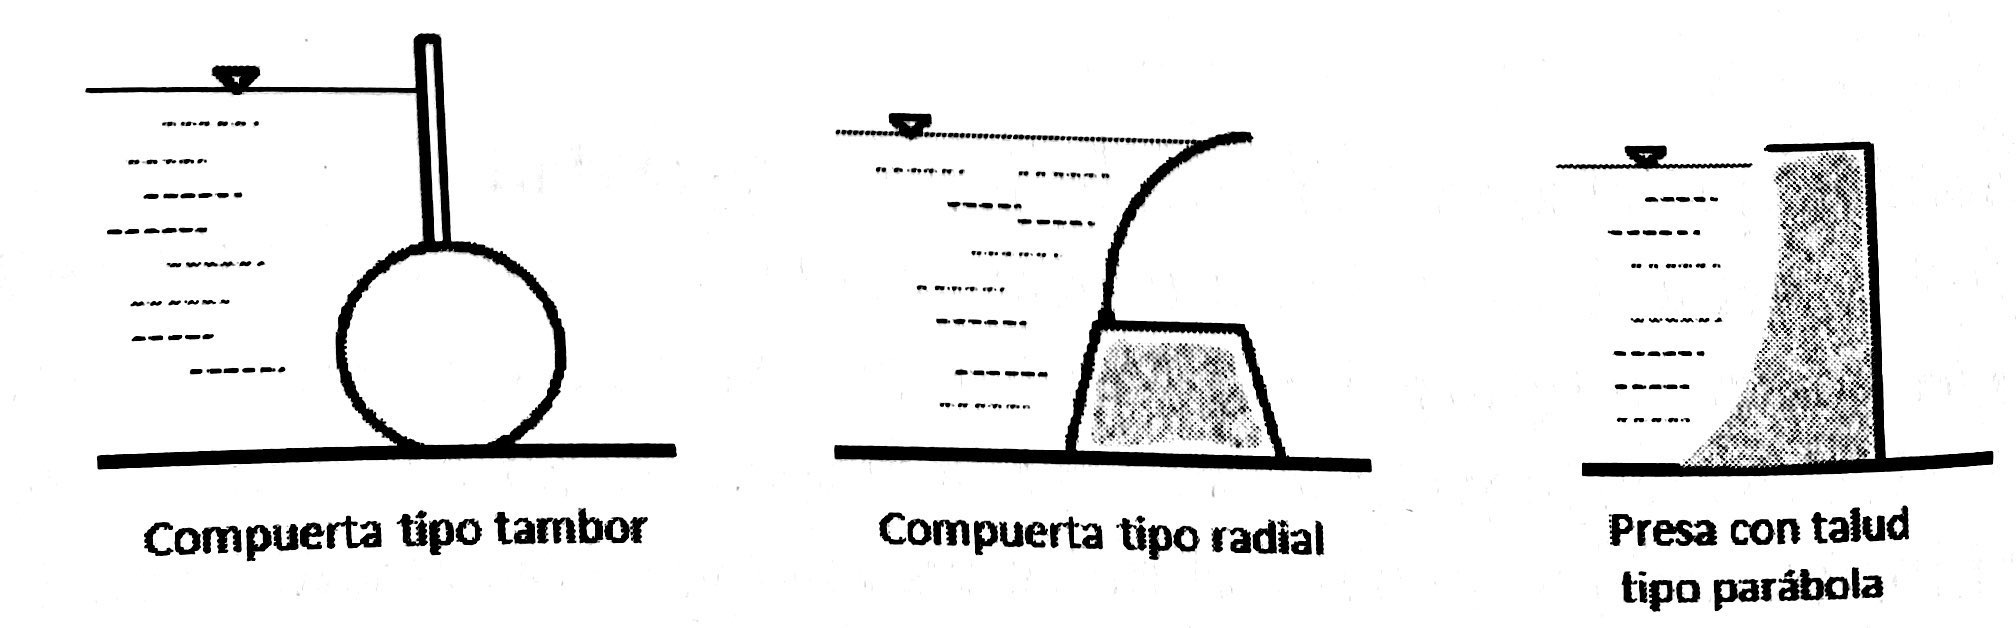
\includegraphics[width=\textwidth]{curb1}
\end{textblock*}
\end{frame} 

\begin{frame}{Fuerzas sobre superficies curvas: Fuerzas}
En una superficie curva sumergida, la fuerza hidroesti\'atica cambia de direccion dependiendo de la posicion sobre la superficie. Para facilitar el calculo, es necesario estimar las componentes horizontal $F_H$ y vertical $F_V$ de  la fuerza resultante $F_R$ sobre la superficie curva. 
\begin{textblock*}{6.5cm}(3.0cm,4.3cm) % {block width} (coords)
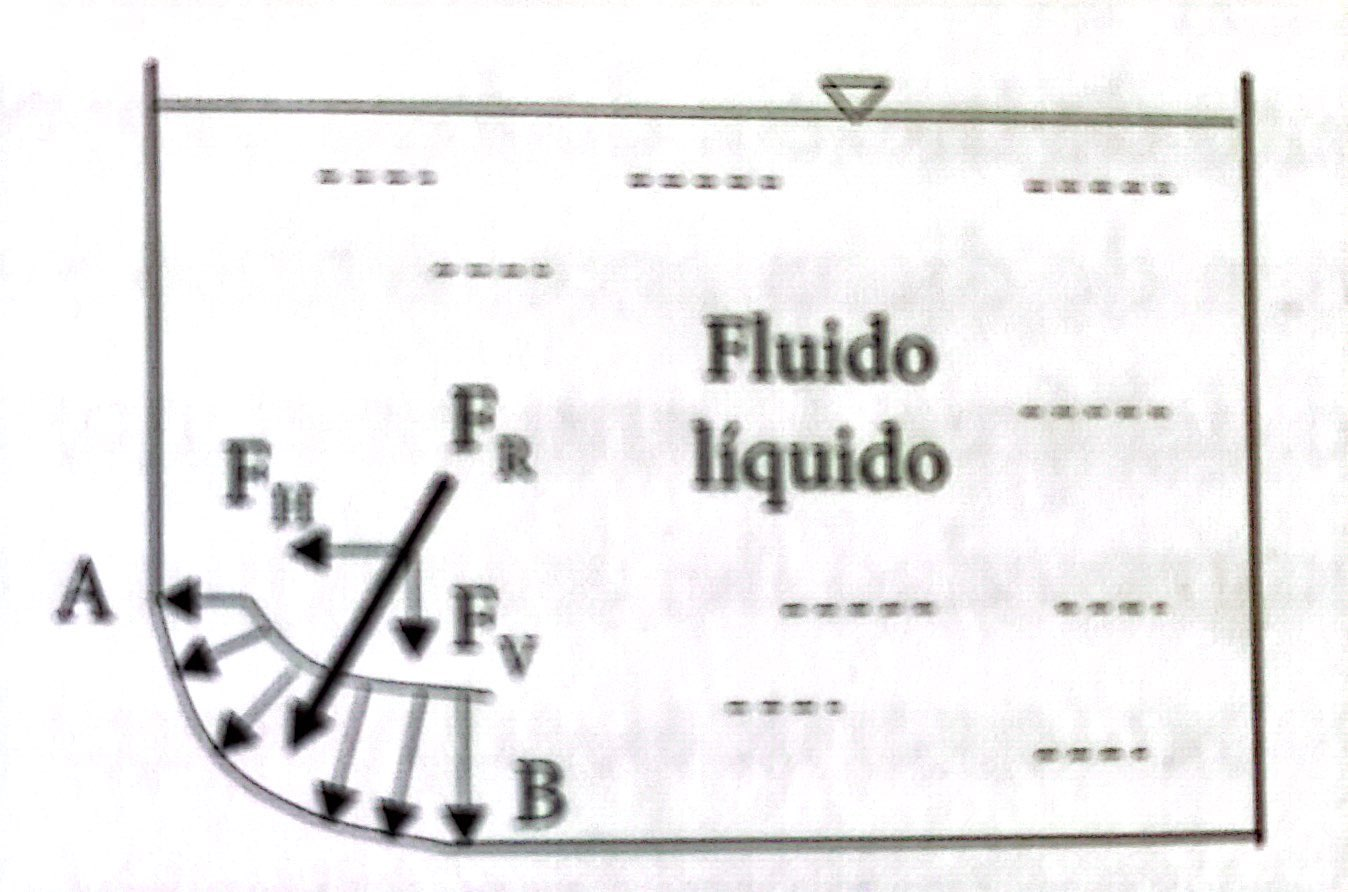
\includegraphics[width=\textwidth]{curb2}
\end{textblock*}
\end{frame}

\begin{frame}{Fuerzas sobre superficies curvas: $F_H$}
\begin{columns}
\column{0.4\textwidth}
La fuerza horizontal $F_H$ sobre la proyecci\'on de la superficie curva es:
$$
F_H=\gamma[h_c A]_{\text{proyecci\'on}} 
$$
\column{0.6\textwidth}
\begin{textblock*}{6cm}(6.8cm,1cm) % {block width} (coords)
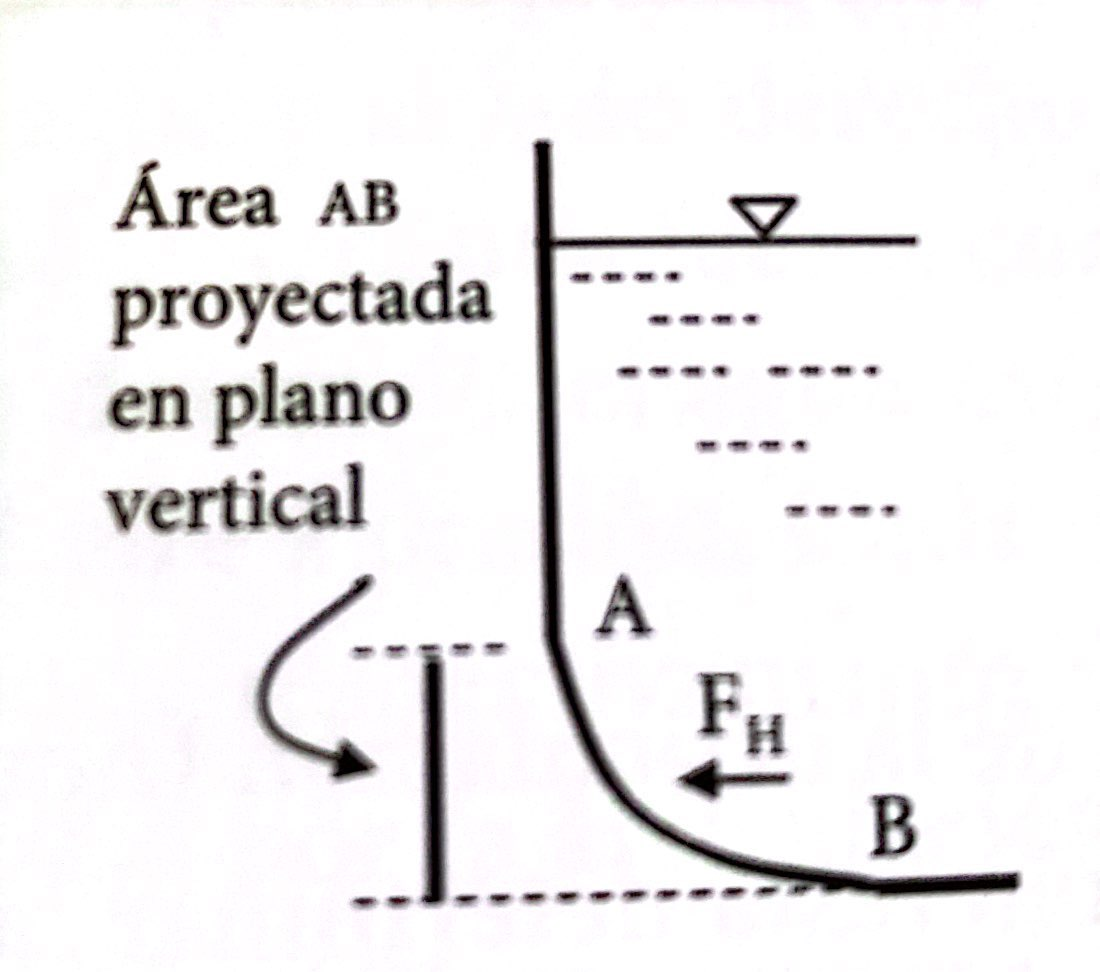
\includegraphics[width=0.9\textwidth]{curb3}
\end{textblock*}
\end{columns}
\vspace{1.5cm}
donde:
\begin{itemize} 
\item $\gamma$: Peso espec\'ifico del fluido en reposo.
\item $h_c$: distancia vertical medida desde la superficie hasta el centro de gravedad de la superficie proyectada
\item $A$: Area de la superficie proyectada sobre el plano vertical.
\end{itemize}
\end{frame}

\begin{frame}{Fuerzas sobre superficies curvas:$y_p$ y $x_p$ para $F_H$}
Como $F_H$ se aplica en el centro de presiones $p$ del area proyectada en un plano vertical, se tiene:
$$
y_p = \left[ y_c + \frac{\bar{I}_c}{y_c A} \right]_{\text{proyecci\'on}}
$$

$$
x_p = \left[ x_c + \frac{\bar{I}_{xy}}{x_c A} \right]_{\text{proyecci\'on}}
$$
donde
\begin{itemize}
\item $\bar{I}_c$: Momento de inercia con respecto al centro de gravedad del area proyectada en un plano vertical.
\item $\bar{I}_{xy}$: Producto de inercia con respecto al centro de gravedad del area proyectada en un plano vertical.
\item $x_c$ y $y_c$ son las coordenadas del centro de gravedad del area proyectada en un plano vertical.
\end{itemize}
\end{frame}

\begin{frame}{Fuerzas sobre superficies curvas: $F_V$}
\begin{columns}
\column{0.6\textwidth}
La componente vertical $F_V$ se calcula como el peso del fluido que esta por encima (fisicamente o no). 
$$
F_V = \gamma [V]_{arriba}
$$
\column{0.4\textwidth}
\begin{textblock*}{3cm}(8cm,1.1cm) % {block width} (coords)
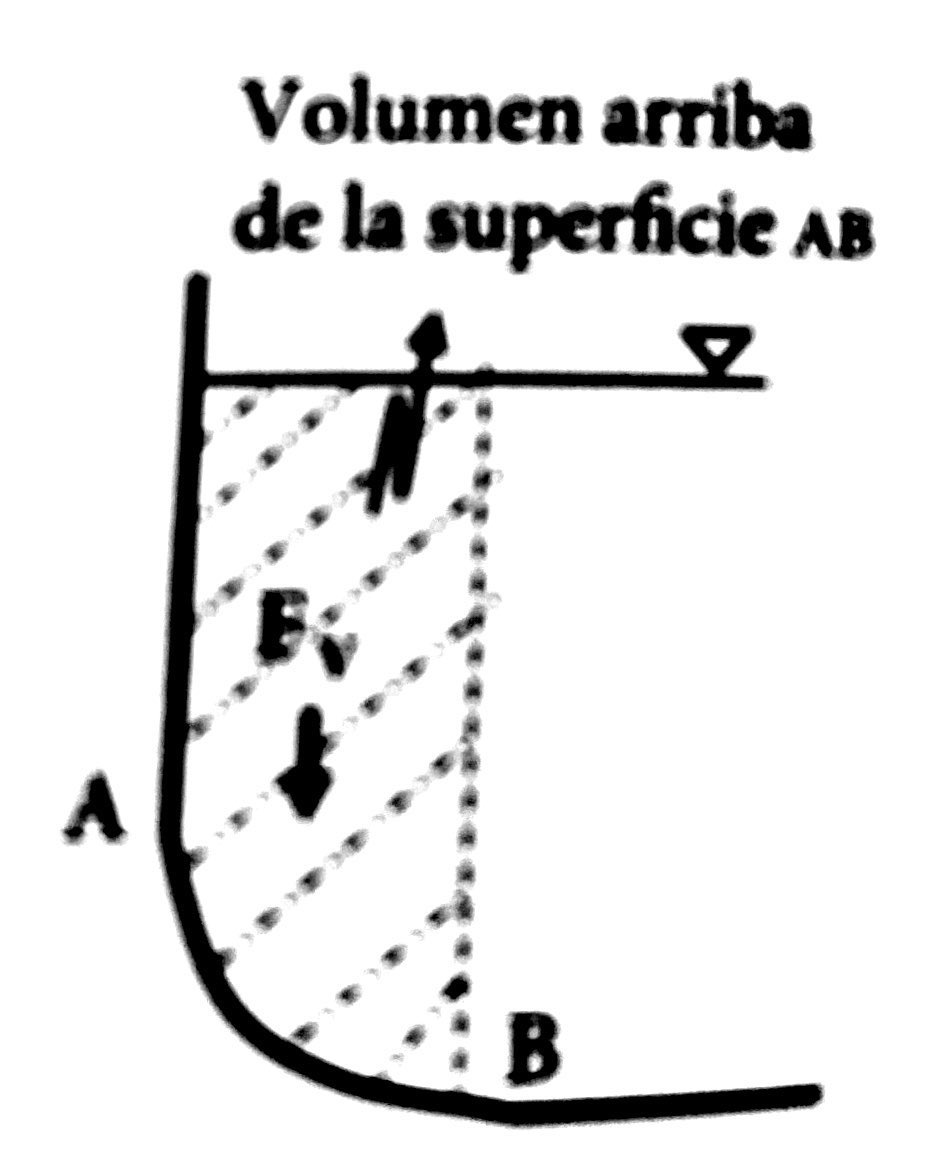
\includegraphics[width=0.9\textwidth]{curb4}
\end{textblock*}
\end{columns}
\vspace{0.8cm}
El punto de aplicaci\'on de $F_V$ es el centro de gravedad del volumen situado arriba de la superficie curva:
$$
y_p = [y_c ]_{V_{arriba}} = \frac{\int_V y dV}{\int_V dV}
$$
$$
x_p = [x_c ]_{V_{arriba}}= \frac{\int_V x dV}{\int_V dV}
$$
Finalmente,la magnitud de la fuerza $F_R$ se calcula como:
$$
\sqrt{F_H^2 + F_V^2}
$$
\end{frame}

%\item $F_x$ se calcula como la resultante de la fuerza hidroestatica sobre una superficie plana vertical $F_x = \gamma\ h_c \ A$
%\item $F_y$ es la fuerza en $y$ ejercida sobre el fluido (e.g. fluido superior y aire) 
%\item $W = \rho g V$ es el peso del volumen ($V$) de fluido. Note que $F_y$ y $W$ se suman si actuan en la misma direccion y se restan si van en direcciones opuestas. 
%\end{itemize}
%$F_R$ se calcula como:
%$$
%F_R=\sqrt{F^2_H + F^2_V}
%$$
%El angulo que hace $F_R$ con la horizontal es:
%$$$
%\alpha = \arctan \frac{F_V}{F_H}
%$$

\section{Fuerzas hidroest\'aticas con diferentes fluidos}
\begin{frame}{Fuerzas hidroest\'aticas con diferentes fluidos}
\begin{columns}
\column{0.4\textwidth}
Las ecuaciones  vistas hasta le momento son validas para fluidos de densidad uniforme. Si el fluido esta conformado por capas de fluidos de diferentes densidades, la distribucion lineal de presiones cambia en cada capa. 
% Fig 3.39 Cengel
\column{0.6\textwidth}
\begin{textblock*}{6cm}(6cm,1.5cm) % {block width} (coords)
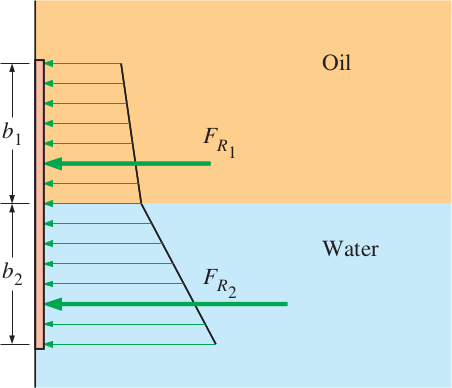
\includegraphics[width=\textwidth]{mden}
\end{textblock*}
\end{columns}
\end{frame}

\begin{frame}{Fuerzas hidroest\'aticas con diferentes fluidos}
Sin embargo las ecuaciones vistas anteriormente pueden ser aplicadas a cada capa $i$ y las $F_{R,i}$ pueden ser adicionadas para calcular la $F_R$:
$$
F_R = \sum F_{R,i} = \sum P_{C,i}A_i
$$
dondei: 
\begin{itemize}
\item $P_{C,i} =  P_0 + \rho_i h_{C,i}$ es la presion en el centroide de la porcion de la superficie en el fluido $i$.
\item $A_i$ es el area de la superficie en ese fluido. El centro de presion de $F_R$ puede ser encontrado calculando la suma de los momentos de cada fuerza $F_{R,i}$ con respecto a un punto determinado (e.g. la superficie de agua).
\end{itemize}
$$
y_p = \frac{\sum F_{R,i}\ y_{p,i}}{F_R} \hspace{1cm} x_p = \frac{\sum F_{R,i}\ x_{p,i}}{F_R}
$$
\end{frame}

\section{Principios de flotacion}
\section{Equilibrio relativo de fluidos en movimiento}


\end{document}

